\documentclass[11pt,a4paper]{article}

% ── Encoding & font ──────────────────────────────────────────────────────────
\usepackage[utf8]{inputenc}
\usepackage[T1]{fontenc}
\usepackage{lmodern}
\usepackage{microtype}

% ── Layout ───────────────────────────────────────────────────────────────────
\usepackage[top=2.2cm, bottom=2.2cm, left=2.4cm, right=2.4cm]{geometry}
\usepackage{parskip}
\setlength{\parindent}{0pt}
\setlength{\parskip}{6pt}

% ── Colors ───────────────────────────────────────────────────────────────────
\usepackage[table]{xcolor}
\definecolor{Teal}{HTML}{2E9D8F}
\definecolor{Purple}{HTML}{7B5EA7}
\definecolor{Coral}{HTML}{E8735A}
\definecolor{TealLight}{HTML}{E6F4F2}
\definecolor{PurpleLight}{HTML}{F0EBF8}
\definecolor{CoralLight}{HTML}{FDF0EC}
\definecolor{GrayLight}{HTML}{F3F4F6}
\definecolor{GrayMid}{HTML}{9CA3AF}
\definecolor{Dark}{HTML}{1F2937}
\definecolor{ChapterBar}{HTML}{1E3A5F}

% ── TikZ ─────────────────────────────────────────────────────────────────────
\usepackage{tikz}
\usetikzlibrary{arrows.meta, positioning, fit, backgrounds, shapes}

% ── Tables ───────────────────────────────────────────────────────────────────
\usepackage{booktabs}
\usepackage{tabularx}
\usepackage{array}
\usepackage{colortbl}
\usepackage{longtable}

% ── Boxes ────────────────────────────────────────────────────────────────────
\usepackage[most]{tcolorbox}

% ── Section headers ──────────────────────────────────────────────────────────
\usepackage{titlesec}
\titleformat{\section}[block]
  {\large\bfseries\color{white}}
  {}
  {0em}
  {\colorbox{ChapterBar}{\parbox[c][1em]{\dimexpr\linewidth-2\fboxsep\relax}{\strut\enspace\thesection\enspace #1}}}

\titleformat{\subsection}[block]
  {\normalsize\bfseries\color{Teal}}
  {}{0em}{}
  [\vspace{-4pt}\color{Teal}\hrule height 0.8pt\vspace{2pt}]

% ── Misc ─────────────────────────────────────────────────────────────────────
\usepackage{enumitem}
\usepackage{fancyhdr}
\setlength{\headheight}{22pt}
\usepackage{float}
\usepackage{amsmath}

\pagestyle{fancy}
\fancyhf{}
\fancyhead[L]{\small\textcolor{GrayMid}{PCOS Research System}}
\fancyhead[R]{\small\textcolor{GrayMid}{Yale University --- Computational Biomedical AI}}
\fancyfoot[C]{\small\textcolor{GrayMid}{\thepage}}
\renewcommand{\headrulewidth}{0.4pt}
\renewcommand{\headrule}{\hbox to\headwidth{\color{Teal}\leaders\hrule height \headrulewidth\hfill}}

% ── Custom environments ───────────────────────────────────────────────────────
\newtcolorbox{concept}[1]{
  colback=TealLight, colframe=Teal, boxrule=1pt,
  title={\small\bfseries #1}, fonttitle=\color{white},
  colbacktitle=Teal, left=8pt, right=8pt, top=5pt, bottom=5pt
}

\newtcolorbox{notebox}{
  colback=CoralLight, colframe=Coral, boxrule=0.8pt,
  left=8pt, right=8pt, top=4pt, bottom=4pt
}

% ── TikZ global styles ────────────────────────────────────────────────────────
\tikzset{
  box/.style={
    rectangle, rounded corners=4pt,
    text width=#1, align=center,
    inner sep=7pt, font=\small
  },
  box/.default=3cm,
  arr/.style={-{Stealth[length=5pt]}, line width=1.2pt, color=GrayMid},
  tArr/.style={-{Stealth[length=5pt]}, line width=1.4pt, color=Teal},
  pArr/.style={-{Stealth[length=5pt]}, line width=1.4pt, color=Purple},
}

% ─────────────────────────────────────────────────────────────────────────────
\begin{document}
\thispagestyle{empty}

% ── COVER ────────────────────────────────────────────────────────────────────
\begin{tikzpicture}[remember picture, overlay]
  \fill[ChapterBar] (current page.north west)
    rectangle ([yshift=-5cm]current page.north east);
  \fill[Teal] ([yshift=-5cm]current page.north west)
    rectangle ([yshift=-5.5cm]current page.north east);
\end{tikzpicture}

\vspace*{1.2cm}
{\color{white}\fontsize{28}{34}\selectfont\bfseries PCOS Research System}\\[0.5cm]
{\color{white}\fontsize{15}{20}\selectfont Building a Computational Biomedical AI Pipeline}\\[0.3cm]
{\color{Teal!60!white}\fontsize{11}{14}\selectfont From API Ingestion to Autonomous Scientific Discovery}

\vspace{3.5cm}

\begin{tcolorbox}[colback=GrayLight, colframe=GrayMid!50, boxrule=0.8pt,
  left=14pt, right=14pt, top=10pt, bottom=10pt]
{\normalsize\color{Dark}
This document is a \textbf{technical reference} for the PCOS computational
research system built at Yale. It explains, in order, every component of the
system: what it does, how it works, and why it was designed that way. It also
explains how to build a \textbf{Claude Code Skill} from scratch.

\vspace{6pt}
\textbf{Topics covered:} Data ingestion from scientific APIs $\cdot$
ETL pipeline $\cdot$ Vector embeddings $\cdot$ LLM classification and extraction $\cdot$
Entity normalization (4-layer architecture) $\cdot$ Anomaly detection $\cdot$
Autonomous research agent (ReAct loop, 6 tools) $\cdot$ Building a Claude Code Skill.
}
\end{tcolorbox}

\vspace{0.8cm}
{\small\color{GrayMid} Yale University $\cdot$ Computational Biomedical AI $\cdot$ April 2026}

\newpage
\tableofcontents
\newpage

% =============================================================================
\section{Data Ingestion --- Fetching Scientific Literature}
% =============================================================================

The system starts by pulling raw data from three external scientific databases.
Each one contributes something different, and together they form the knowledge
base the AI will learn from.

\subsection{The Three Data Sources}

\begin{figure}[H]
\centering
\begin{tikzpicture}

% Three source boxes at fixed coordinates
\node[box=4.2cm, fill=TealLight, draw=Teal, line width=1pt] at (0,0) (pm) {
  \textbf{PubMed}\\[3pt]
  {\footnotesize\normalfont NCBI E-utilities API\\
  \textit{esearch} (get IDs) + \textit{efetch} (get abstracts)\\
  Rate limit: 10 req/s with API key\\
  Format: XML $\rightarrow$ parsed to JSON}
};

\node[box=4.2cm, fill=TealLight, draw=Teal, line width=1pt] at (5.5,0) (oa) {
  \textbf{OpenAlex}\\[3pt]
  {\footnotesize\normalfont Open-source academic API\\
  Adds: citation counts, co-authors,\\
  semantic concept labels\\
  Format: JSON, cursor pagination}
};

\node[box=4.2cm, fill=TealLight, draw=Teal, line width=1pt] at (11,0) (ct) {
  \textbf{ClinicalTrials.gov}\\[3pt]
  {\footnotesize\normalfont U.S. registry of clinical trials\\
  API v2 (2023)\\
  Fields: phase, status, enrollment,\\
  interventions, outcome measures}
};

% Output arrow
\node[box=10cm, fill=GrayLight, draw=GrayMid, line width=0.8pt] at (5.5,-3.2) (out) {
  \textbf{Output:} \texttt{data/raw/*.jsonl} \quad (one JSON object per line)\\[3pt]
  {\footnotesize\normalfont JSONL = JSON Lines. Each line is a valid, independent JSON record.
  The format allows reading files line-by-line without loading everything into memory.}
};

\end{tikzpicture}
\caption{The three data sources and their output format}
\end{figure}

\subsection{What is a REST API?}

A \textbf{REST API} (Representational State Transfer Application Programming Interface)
is a standard way to communicate with a remote server over the internet.
Your Python script sends an \textbf{HTTP GET request} with parameters, and the server
responds with structured data (usually JSON or XML).

\begin{tcolorbox}[colback=PurpleLight, colframe=Purple, boxrule=0.8pt,
  left=8pt, right=8pt, top=5pt, bottom=5pt, title={\small\bfseries Example: PubMed ESearch call},
  fonttitle=\color{white}, colbacktitle=Purple]
{\small\ttfamily
GET https://eutils.ncbi.nlm.nih.gov/entrez/eutils/esearch.fcgi\\
\quad ?db=pubmed\&term=polycystic+ovary+syndrome[MeSH]\&retmax=10000

\vspace{4pt}
\normalfont\small
Response: a list of PMIDs (PubMed IDs). Then a second call to EFetch retrieves
the full abstract, authors, journal, and year for each ID.
}
\end{tcolorbox}

\subsection{Rate Limiting and Idempotency}

\textbf{Rate limiting} is a server-side restriction on how many requests you can make per
second. PubMed allows 10 requests/second with an API key; without one, only 3/second.
The scripts use \texttt{time.sleep(0.1)} between requests to stay within limits.

\textbf{Idempotency} means running a script multiple times produces the same result as
running it once. All ingestion scripts use \texttt{INSERT OR IGNORE} in SQLite ---
if an article already exists, it is silently skipped. This makes reruns safe.

% =============================================================================
\section{The Knowledge Base --- ETL, SQLite, and ChromaDB}
% =============================================================================

Raw JSONL files are useful for storage, but not for querying. The ETL step
normalizes and loads everything into two complementary databases.

\subsection{ETL: Extract, Transform, Load}

\textbf{ETL} is the foundational pattern of data engineering. Every data pipeline
that moves information from one system to another follows this structure:

\begin{figure}[H]
\centering
\begin{tikzpicture}

\node[box=3cm, fill=TealLight, draw=Teal] at (0,0) (e) {
  \textbf{Extract}\\[3pt]
  {\footnotesize\normalfont Read raw JSONL files from \texttt{data/raw/}}
};
\node[box=3.5cm, fill=PurpleLight, draw=Purple] at (5,0) (t) {
  \textbf{Transform}\\[3pt]
  {\footnotesize\normalfont Normalize fields, deduplicate by PMID/DOI, compute evidence score}
};
\node[box=3cm, fill=CoralLight, draw=Coral] at (10.2,0) (l) {
  \textbf{Load}\\[3pt]
  {\footnotesize\normalfont INSERT into SQLite. UPSERT into ChromaDB}
};

\end{tikzpicture}
\caption{The ETL pattern applied in \texttt{build\_knowledge\_base.py}}
\end{figure}

\subsection{SQLite --- Structured Data}

\textbf{SQLite} is a relational database stored in a single file (\texttt{pcos\_research.db}).
It supports full SQL and is ideal for projects where a single process writes data.
Its critical constraint: \textbf{only one writer at a time}. This is why the entire
pipeline must run sequentially, never in parallel.

Two important SQLite settings used throughout the project:

\begin{itemize}[noitemsep]
\item \texttt{PRAGMA journal\_mode=WAL} --- Write-Ahead Logging mode, which allows
  readers (SELECT queries) to run simultaneously with a writer (INSERT), preventing
  read locks.
\item \texttt{connection timeout=60} --- If the database is locked by another process,
  wait up to 60 seconds before raising an error, rather than failing immediately.
\end{itemize}

The database has seven tables: \texttt{articles}, \texttt{article\_llm\_labels},
\texttt{article\_extractions}, \texttt{entity}, \texttt{article\_entity\_links},
\texttt{intervention\_signals}, and \texttt{clinical\_trials}. The relationships
between them form a knowledge graph of interventions, populations, and outcomes.

\subsection{ChromaDB --- Semantic Search}

\textbf{ChromaDB} is a \textbf{vector database}: instead of storing text, it stores
numerical \textbf{embeddings} --- lists of 768 numbers that encode the meaning of
a text. When you search ChromaDB, you do not search for exact words; you search
for \textit{meaning}, and it returns the most semantically similar documents.

\begin{concept}{What is an Embedding?}
An embedding is a representation of text as a point in high-dimensional space.
Two texts about similar topics will have points that are close together.
This is computed by a model called \textbf{nomic-embed-text}, which runs locally via
Ollama. The 768-dimensional space means each text becomes a list of 768 numbers,
where numbers at similar positions encode similar semantic features.
\end{concept}

The similarity between two embeddings is measured with \textbf{cosine similarity}:
a value between 0 (unrelated) and 1 (identical meaning). ChromaDB's internal index
uses the \textbf{HNSW algorithm} (Hierarchical Navigable Small World) to find the
nearest neighbors in milliseconds, even across 12,155 vectors.

% =============================================================================
\section{AI Processing --- Labeling, Extraction, and Schema v1.1}
% =============================================================================

The pipeline has two LLM-powered steps that convert free-form abstracts into
structured scientific data.

\subsection{Step 1: Classification (Labeling)}

The classifier reads each article's title and abstract and assigns three fields.
This is a \textbf{few-shot prompting} task: the prompt includes 4--5 labeled examples
so Gemma understands the expected format and standard.

\rowcolors{2}{GrayLight}{white}
\begin{tabularx}{\linewidth}{>{\bfseries\small}p{3.2cm} >{\small}p{2.8cm} >{\small}X}
\toprule
\rowcolor{Teal!15}
\textbf{Field} & \textbf{Values} & \textbf{Meaning} \\
\midrule
study\_type\_llm & RCT, meta-analysis, cohort, case study, narrative\ldots & What kind of study is this? \\
evidence\_tier\_llm & tier\_1 to tier\_4 & Quality level (1 = gold standard, 4 = opinion) \\
utility\_score\_llm & 0.0 -- 1.0 & How relevant is this article to PCOS research? \\
\bottomrule
\end{tabularx}

\subsection{Step 2: Structured Extraction (Schema v1.1)}

The extractor is more demanding: it reads each abstract and fills out a structured
record with specific scientific fields. Version 1.1 adds five new \textbf{population
subgroup fields}, which are critical for detecting subpopulation variance.

\begin{figure}[H]
\centering
\begin{tikzpicture}

\node[box=4.5cm, fill=GrayLight, draw=GrayMid] at (0,0) (in) {
  \textbf{Input: article abstract}\\[3pt]
  {\footnotesize\normalfont Free-form scientific text with no structure}
};

\node[box=4.8cm, fill=PurpleLight, draw=Purple] at (6.5,0) (llm) {
  \textbf{Gemma 4 --- Extractor mode}\\[3pt]
  {\footnotesize\normalfont temperature = 0 (deterministic)\\
  num\_predict = 600 tokens\\
  Prompt: PICO-formatted schema}
};

\node[box=4.5cm, fill=TealLight, draw=Teal] at (0,-3.5) (s1) {
  \textbf{Study fields}\\[3pt]
  {\footnotesize\normalfont study\_type, sample\_size,\\
  duration\_weeks, intervention,\\
  comparator, dose,\\
  effect\_direction, effect\_magnitude}
};

\node[box=4.8cm, fill=CoralLight, draw=Coral] at (6.5,-3.5) (s2) {
  \textbf{Population fields (v1.1)}\\[3pt]
  {\footnotesize\normalfont population\_diet (e.g. ``Mediterranean diet'')\\
  population\_bmi (e.g. ``obese BMI\textgreater 30'')\\
  population\_age\_range\\
  population\_comorbidities\\
  population\_ethnicity}
};

\end{tikzpicture}
\caption{Extraction schema v1.1 --- study fields and new population fields}
\end{figure}

\begin{notebox}
\textbf{Why do population fields matter?} Without them, you can only say
``berberine works in 8 of 10 studies.'' With them, the anomaly scanner can discover
that berberine works in 6/6 studies with obese patients, but only 2/4 with
normal-weight patients --- a subpopulation signal invisible without this data.
\end{notebox}

\textbf{Prioritization}: the extractor does not process all 12,155 articles at once.
It selects those with \texttt{evidence\_tier\_llm = 'tier\_1'} and high
\texttt{utility\_score\_llm} first, maximizing the scientific return per LLM call.

% =============================================================================
\section{Entity Normalization --- 4-Layer Architecture}
% =============================================================================

Drug names in scientific papers are inconsistent. The same compound appears as
``metformin'', ``Metformin HCl'', ``metformin 1500 mg/day'', and ``glucophage''.
Without normalization, these are treated as different entities and their statistics
cannot be aggregated. The entity normalizer solves this.

\subsection{The Problem and Solution}

\begin{concept}{Canonical Entity}
A \textbf{canonical entity} is the single, official name chosen to represent all
variant spellings. The normalizer maps every raw term found in a paper back to its
canonical name. The system maintains a \textbf{SEED dictionary} --- a curated Python
dict of 76+ canonical entities with their known aliases.
\end{concept}

\subsection{The 4-Layer Pipeline}

Each raw term passes through layers in order, stopping at the first successful match.

\begin{figure}[H]
\centering
\begin{tikzpicture}

% All nodes centered at x=4.5, stacked vertically — no overlaps

\node[box=4.5cm, fill=GrayLight, draw=GrayMid] at (4.5,7.2) (in) {
  \textbf{raw\_term} {\footnotesize\normalfont from paper}\\[2pt]
  {\footnotesize e.g. ``Metformin 1500 mg/day oral tablet''}
};

\node[box=9cm, fill=CoralLight, draw=Coral] at (4.5,5.5) (noise) {
  \textbf{NOISE FILTER (pre-check)}\\[2pt]
  {\footnotesize\normalfont
  NOISE\_TERMS: ``placebo'', ``pcos'', ``serum'', ``control group'', ``ogtt''\ldots $\approx$40 terms\\
  len $<$ 3 · NOISE\_SUBSTRINGS: ``questionnaire'', ``assessment tool''\ldots\\
  $\rightarrow$ if noise: \textbf{SKIP}}
};

\node[box=9cm, fill=TealLight, draw=Teal, line width=1.2pt] at (4.5,3.7) (l1) {
  \textbf{Layer 1 --- Exact Match in SEED aliases}\\[2pt]
  {\footnotesize\normalfont
  O(1) dict lookup across 76+ canonical entities and all their known aliases.\\
  ``glucophage'' $\rightarrow$ alias of ``metformin'' $\rightarrow$
  \textbf{method=exact, confidence=1.0}}
};

\node[box=9cm, fill=TealLight, draw=Teal] at (4.5,2.0) (l2) {
  \textbf{Layer 2 --- Fuzzy Matching (rapidfuzz WRatio)}\\[2pt]
  {\footnotesize\normalfont
  FUZZY\_CUTOFF=80 · FUZZY\_HIGH\_CONF=93\\
  score $\geq$ 93 $\rightarrow$ \textbf{method=fuzzy} \qquad
  score 80--93 $\rightarrow$ Layer 2.5 \qquad
  score $<$ 80 $\rightarrow$ Layer 3}
};

\node[box=9cm, fill=PurpleLight, draw=Purple] at (4.5,0.3) (l25) {
  \textbf{Layer 2.5 --- LLM Verification (score 80--93)}\\[2pt]
  {\footnotesize\normalfont
  Gemma: ``choose from [candidate, alt1, alt2] or `none'\,''\\
  YES $\rightarrow$ \textbf{method=fuzzy\_verified} \qquad NO $\rightarrow$ Layer 3}
};

\node[box=9cm, fill=PurpleLight, draw=Purple, line width=1.2pt] at (4.5,-1.6) (l3) {
  \textbf{Layer 3 --- LLM Resolution (3-way classification)}\\[2pt]
  {\footnotesize\normalfont
  \textbf{alias} $\rightarrow$ maps to existing entity · raw\_term added as permanent alias · \textbf{method=llm}\\
  \textbf{new} $\rightarrow$ legitimate new drug, inserted as new\_entity (pending human curation)\\
  \textbf{discard} $\rightarrow$ noise that passed the filter, silently dropped}
};

\end{tikzpicture}
\caption{Entity Normalizer v4 --- 4-layer resolution pipeline}
\end{figure}

\subsection{The Alias Learner}

One design feature worth highlighting: when Layer 3 classifies a term as
``alias'', it does two things simultaneously. It creates the entity link
\textit{and} permanently adds the raw term to the SEED aliases.
The next time that term appears in any paper, it is resolved instantly in
Layer 1 --- no LLM call needed. \textbf{The system learns from every run},
progressively reducing the number of LLM calls required.

\subsection{Why Not Use a Standard Medical Ontology?}

Medical ontologies like MeSH or ChEBI contain hundreds of thousands of terms.
Querying them for every unknown term would be slow and would return irrelevant matches.
The curated SEED with 76+ targeted entities covers over 95\% of interventions
that actually appear in PCOS literature --- a much better precision/recall tradeoff.

% =============================================================================
\section{Anomaly Detection --- Signals Without Prior Hypotheses}
% =============================================================================

Most scientific research starts with a hypothesis and tests it. This system
does the opposite: it scans the aggregated data for patterns that \textit{nobody
was looking for}. This is possible because the entity normalizer connects
hundreds of papers through their canonical entities.

\subsection{Three Types of Signal}

\begin{figure}[H]
\centering
\begin{tikzpicture}

\node[box=4cm, fill=CoralLight, draw=Coral, line width=1.2pt] at (0,0) (t1) {
  \textbf{Type 1}\\
  \textit{Cross-Indication}\\[4pt]
  {\footnotesize\normalfont A drug designed for\\
  disease A appears in $\geq$2 PCOS\\
  studies with favorable effect.\\[4pt]
  Example: roflumilast\\
  (designed for COPD)\\
  shows benefit in PCOS RCTs.}
};

\node[box=4cm, fill=CoralLight, draw=Coral, line width=1.2pt] at (5.5,0) (t2) {
  \textbf{Type 2}\\
  \textit{Subpopulation Variance}\\[4pt]
  {\footnotesize\normalfont Same treatment, but effect\\
  is $>$30 percentage points\\
  higher in one subgroup\\
  (diet, BMI, ethnicity).\\[4pt]
  Example: berberine 85\%\\
  favorable in obese vs.\\
  42\% in normal-weight.}
};

\node[box=4cm, fill=CoralLight, draw=Coral, line width=1.2pt] at (11,0) (t3) {
  \textbf{Type 3}\\
  \textit{Unexpected Co-Outcome}\\[4pt]
  {\footnotesize\normalfont An outcome that was not\\
  the study's primary aim\\
  appears repeatedly across\\
  studies of one intervention.\\[4pt]
  Suggests a mechanism\\
  nobody has studied directly.}
};

% Label above
\node[font=\footnotesize\bfseries\color{Dark}, above=0.3cm of t1] {\textit{Drug repurposing}};
\node[font=\footnotesize\bfseries\color{Dark}, above=0.3cm of t2] {\textit{Precision medicine}};
\node[font=\footnotesize\bfseries\color{Dark}, above=0.3cm of t3] {\textit{Hidden mechanism}};

\end{tikzpicture}
\caption{Three types of emergent signal detected by \texttt{anomaly\_scan\_v2.py}}
\end{figure}

\subsection{The Historical Precedent: Metformin}

Metformin was developed in the 1950s for type 2 diabetes. Its use in PCOS emerged
in the 1990s when clinicians noticed that insulin-resistant PCOS patients responded
to it. Today it is the first-line PCOS treatment. The anomaly scanner is designed
to find the \textit{next metformin}: a drug from another field quietly showing
benefit in PCOS data, before any research team explicitly studies it.

% =============================================================================
\section{The Research Agent --- Autonomous Investigation}
% =============================================================================

When the anomaly scanner finds a signal, a human investigator would normally
spend days reading the relevant literature. The research agent does this
autonomously in 5--15 minutes, using a pattern called the \textbf{ReAct loop}.

\subsection{What is an AI Agent?}

A standard LLM answers a question in a single step. An \textbf{AI agent} can
take multiple steps, using \textbf{tools} between them. Each step: reason about
what information is needed, call a tool to get it, observe the result, reason
again. This loop repeats until the agent has enough information to draw a conclusion.

\begin{concept}{ReAct: Reason + Act}
ReAct (Yao et al., 2022) is the foundational pattern for agentic AI.
\textbf{Reason}: the LLM explains what it knows and what it needs.
\textbf{Act}: the LLM invokes a tool (search, SQL, web).
\textbf{Observe}: the tool result is added to the context.
The cycle repeats. The LLM always sees the full history of what it has found so far.
\end{concept}

\subsection{The Six Tools}

\begin{figure}[H]
\centering
\begin{tikzpicture}

% Central agent box
\node[box=4.5cm, fill=PurpleLight, draw=Purple, line width=1.5pt] at (5.5,0) (agent) {
  \textbf{Gemma 4 --- Detective Mode}\\[5pt]
  {\footnotesize\normalfont temperature = 0.15 (exploratory)\\
  num\_predict = 2,000 tokens\\
  num\_ctx = 8,192 tokens\\[3pt]
  max\_steps = 12\\
  Reason $\rightarrow$ Act $\rightarrow$ Observe $\rightarrow$ Reason\ldots}
};

% Tool 1 (top left)
\node[box=3cm, fill=TealLight, draw=Teal] at (0,3.2) (t1) {
  \textbf{semantic\_search}\\
  {\footnotesize\normalfont ChromaDB similarity\\12,155 embeddings}
};

% Tool 2 (top center)
\node[box=3cm, fill=TealLight, draw=Teal] at (5.5,3.2) (t2) {
  \textbf{sql\_query}\\
  {\footnotesize\normalfont SQLite SELECT only\\structured data}
};

% Tool 3 (top right)
\node[box=3cm, fill=TealLight, draw=Teal] at (11,3.2) (t3) {
  \textbf{web\_search}\\
  {\footnotesize\normalfont DuckDuckGo\\mechanisms, context}
};

% Tool 4 (bottom left)
\node[box=3cm, fill=GrayLight, draw=GrayMid] at (0,-3.2) (t4) {
  \textbf{fetch\_abstract}\\
  {\footnotesize\normalfont PubMed EFetch\\full abstract by PMID}
};

% Tool 5 (bottom center)
\node[box=3cm, fill=GrayLight, draw=GrayMid] at (5.5,-3.2) (t5) {
  \textbf{pubmed\_search}\\
  {\footnotesize\normalfont PubMed live query\\papers not in local DB}
};

% Tool 6 (bottom right)
\node[box=3cm, fill=GrayLight, draw=GrayMid] at (11,-3.2) (t6) {
  \textbf{biorxiv\_search}\\
  {\footnotesize\normalfont bioRxiv + medRxiv\\recent preprints}
};

\end{tikzpicture}
\caption{The research agent and its 6 tools. The agent calls each tool and receives its result back into context.}
\end{figure}

\subsection{Tool Use: How the LLM Calls Functions}

\textbf{Tool use} (also called \textit{function calling}) is a capability of modern
LLMs: instead of generating only text, the model can output a structured JSON
object requesting a specific function call. The host code (Python) executes the
function and returns the result as the next message. Ollama supports this natively
via the \texttt{tools} parameter in \texttt{/api/chat}.

\subsection{Why temperature = 0.15?}

For deterministic tasks (extraction, classification), temperature is set to 0 ---
the model always produces the same output for the same input, which is necessary
for reproducibility. The research agent uses 0.15 instead: a small amount of
randomness allows it to explore different investigative paths when the same
signal is investigated multiple times, rather than always following the
identical reasoning chain.

\subsection{The Output}

After up to 12 steps, the agent produces:
a natural-language reasoning trace (the full investigation),
a structured JSON conclusion with a \texttt{mechanistic\_hypothesis},
a \texttt{plausibility\_score} (0.0--1.0),
a list of \texttt{research\_gaps}, and a \texttt{proposed\_experiment}.
The full report is saved to \texttt{reports/research\_agent\_<name>.md}.

% =============================================================================
\section{Building a Claude Code Skill}
% =============================================================================

A \textbf{Claude Code Skill} is a plain-text file that gives Claude a specialized
behavioral mode when a specific command is invoked. It is not code --- it is
\textit{instructions} written in markdown that Claude reads and follows.

\subsection{The File Structure}

Every skill is a single file: \texttt{\textasciitilde/.claude/skills/<skill-name>/SKILL.md}.

\begin{figure}[H]
\centering
\begin{tikzpicture}

% Filesystem tree
\node[box=5cm, fill=GrayLight, draw=GrayMid, text width=5cm, align=left] at (0,0) (tree) {
  \texttt{\small
  \textasciitilde/.claude/skills/\\
  \quad pcos-agent/\\
  \quad \quad SKILL.md \textbf{$\leftarrow$ the only file}\\
  \quad my-other-skill/\\
  \quad \quad SKILL.md
  }
};

% SKILL.md breakdown
\node[box=6.5cm, fill=TealLight, draw=Teal, text width=6.5cm, align=left] at (8.5,1.2) (fm) {
  \textbf{FRONTMATTER (YAML)} --- the ``who am I?''\\[3pt]
  {\footnotesize\normalfont
  \texttt{---}\\
  \texttt{name: pcos-agent}\\
  \texttt{description: >}\\
  \texttt{\quad WHEN to activate this skill.}\\
  \texttt{\quad Keywords and triggers.}\\
  \texttt{---}\\[3pt]
  Claude reads this to decide whether to activate the skill.
  It must contain the trigger phrases the user might say.
  }
};

\node[box=6.5cm, fill=PurpleLight, draw=Purple, text width=6.5cm, align=left] at (8.5,-1.8) (body) {
  \textbf{BODY (Markdown)} --- the ``what do I do?''\\[3pt]
  {\footnotesize\normalfont
  Plain markdown with sections:\\
  $\cdot$ Context: paths, scripts, database info\\
  $\cdot$ How to build the command for each mode\\
  $\cdot$ What to show the user during execution\\
  $\cdot$ How to format the final output\\[3pt]
  Claude follows these instructions exactly when invoked.
  }
};

\end{tikzpicture}
\caption{Anatomy of a SKILL.md file: frontmatter (when to activate) and body (what to do)}
\end{figure}

\subsection{The pcos-agent Skill: Four Modes}

The \texttt{pcos-agent} skill wraps the entire research system into four commands.

\rowcolors{2}{GrayLight}{white}
\begin{tabularx}{\linewidth}{
  >{\bfseries\small\ttfamily}p{3.8cm}
  >{\small}X
  >{\small\color{GrayMid}}p{3.5cm}}
\toprule
\rowcolor{Teal!15}
\textbf{Command} & \textbf{What it does} & \textbf{Runs} \\
\midrule
/pcos-agent investigate \textit{entity} &
  Launches Gemma 4 as a detective scientist. Runs the full ReAct loop with 6 tools
  to investigate a drug or supplement in PCOS context. Produces a mechanistic hypothesis. &
  \texttt{research\_agent.py\newline --entity} \\

/pcos-agent scan &
  Runs the anomaly scanner on the full database. Detects cross-indication signals,
  subpopulation variance, and unexpected co-outcomes. Shows results in a formatted table. &
  \texttt{anomaly\_scan\_v2.py} \\

/pcos-agent status &
  Queries the database and shows key statistics: article counts by tier, top
  interventions by study count, and a list of recent research reports. &
  Python inline SQL \\

/pcos-agent review \textit{name} &
  Reads an existing research report from \texttt{reports/} and presents
  the key findings: plausibility, hypothesis, evidence, gaps. &
  Read tool on .md file \\
\bottomrule
\end{tabularx}

\subsection{Design Principles of a Good Skill}

A skill is only as useful as how completely it briefs Claude.
The body of \texttt{SKILL.md} must be \textbf{self-contained}: Claude cannot
``look around'' in your filesystem to find paths, scripts, or data locations ---
every piece of information it needs must be written explicitly in the skill.

\begin{tcolorbox}[colback=CoralLight, colframe=Coral, boxrule=0.8pt,
  left=8pt, right=8pt, top=5pt, bottom=5pt]
\textbf{Bad skill body:} ``Execute the research script.''\\[4pt]
\textbf{Good skill body:} ``Run \texttt{.venv/Scripts/python.exe scripts/research\_agent.py
--entity [X] --max-steps 12} from the directory
\texttt{C:\textbackslash Users\textbackslash emaza\textbackslash OneDrive\textbackslash Escritorio\textbackslash CODEX\textbackslash PRUEBA1}.
The venv is at \texttt{.venv/Scripts/python.exe} (not system Python). The output
is printed to stdout and saved to \texttt{reports/research\_agent\_<name>.md}.''
\end{tcolorbox}

\end{document}
